\section{Hyperparameters for Soft Actor Critic Training}

% SAC training workflow
In the paper which proposed the soft actor critic alorithm \cite{haarnoja2018soft}, a workflow is presented as Figure \ref{fig:sac_algorithm}.

  \begin{figure}[H]
      \centering
      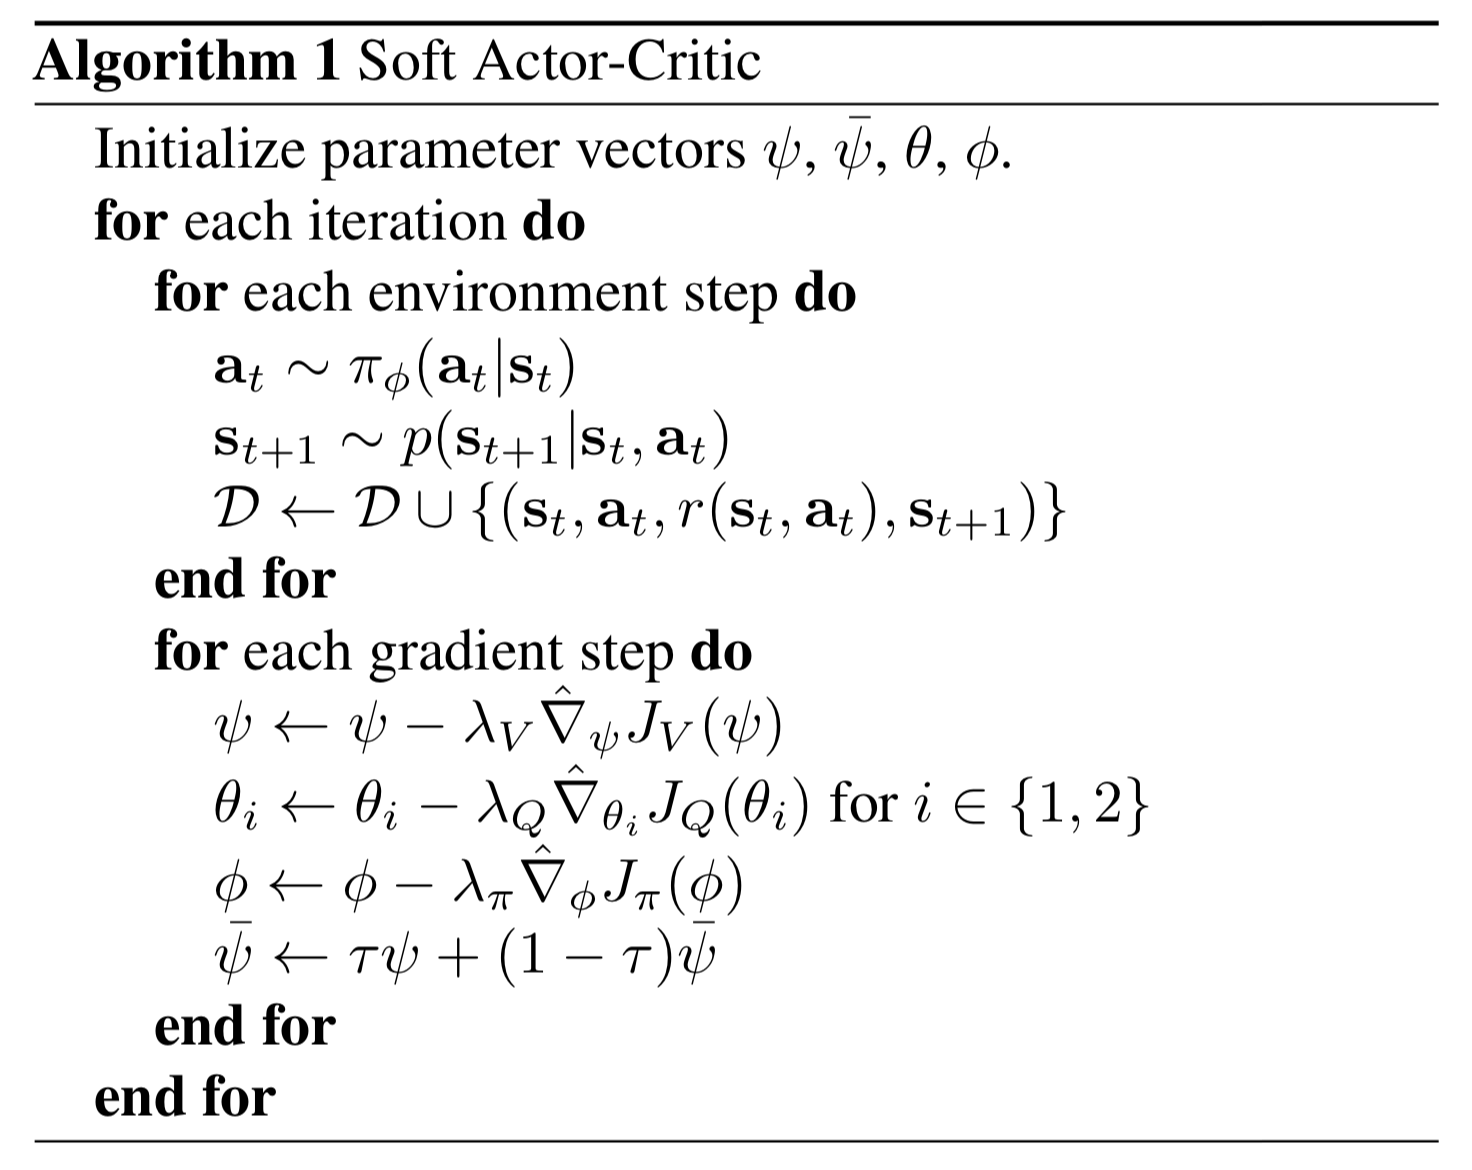
\includegraphics[width=1\textwidth]{figures/external/sac_algorithm.png}
      \caption{Soft Actor Critic algorithm as seen in \cite{haarnoja2018soft}}
      \label{fig:sac_algorithm}
  \end{figure}

The soft actor critic algorithm consists of 3 deep neural networks: a state value function $V$, a state-action value function $Q$, and a policy $\pi$. In \ref{fig:sac_algorithm}, the parameters of the functions, or in this case their weight values, are set as $\psi$, $\theta$, and $\phi$ respectively. Each deep neural network has one hidden layer that consists of 256 neurons.

The learning rates of each deep neural network are set as the following.
  \begin{itemize}
    \item $\lambda_V = 3.0 \times 10^{-4}$
    \item $\lambda_Q = 3.0 \times 10^{-4}$
    \item $\lambda_\pi = 3.0 \times 10^{-4}$
    \item $\tau = 5.0 \times 10^{-3}$
  \end{itemize}


We trained our policies using batch training, where we preserve a set size of trajectories, or replay buffer size, of states and actions taken by the policy per iteration. Parameters regarding batch training are set as the following.
  \begin{itemize}
    \item Iterations (epochs): 3000
    \item Environment steps per iteration: 1000
    \item Gradient steps per iteration: 1000
    \item Batch size: 256
    \item Replay buffer size: $1.0 \times 10^6$
  \end{itemize}

Trajectories of states and actions totaling 5000 steps per epoch for determining the average return for evaluation.

Returns $R$ are calculated as the following,
  \begin{equation}
    R = \sum_{t = 0}^n \gamma^t r_t
  \end{equation}
  where $r_t$ is the reward gained during timestep $t$, $n$ is the total number of timesteps taken to calculate $R$, and $\gamma$ is the discount. For all of our experiments, we set $\gamma = 0.99$.
